Consider the quadrature-oscillator circuit given Fig. \ref{fig:es17btech11009_fig1} without the limiter. Let the resistance $R_{f}$ be equal to $\frac{2R}{1 + \Delta}$ where $\Delta << 1$. Show that the poles of the characteristic equation are in the right-half s plane and given by 
s $\approx \frac{1}{CR}(\frac{\Delta}{4}\pm j)$

\numberwithin{equation}{enumi}
\begin{figure}[!ht]
\begin{center}
\resizebox{\columnwidth}{!}{\begin{circuitikz}
\ctikzset{bipoles/length=1cm}
 \ctikzset{
amplifiers/fill=cyan
}
 
\draw (0, 0) node[op amp] (opamp) {\texttt{2}};
\draw (opamp.-) --(-1,0.35)-- (-1,1.25) to[R=$2R$,*-*] (1,1.25) -- (1,0) -- (1,-1.25) to  [vR=$R_{f}$,*-*] (-1,-1.25) -- (-1,-0.35) to (opamp.+);
\draw (-1,-1.25) to[C=$C$,*-*] (-1, -3) to node[ground]{} (-1,-3);
\draw (opamp.out) --(1,0) ;
\draw (-5,-1.25) node[op amp](opamp2){\texttt{1}};
\draw (-1,-1.25) to [R=$2R$,*-*](-4,-1.25) to (opamp2.out);
\draw (opamp2.-) --(-7.5,-0.9) to [R=$R$,*-*](-9.5,-0.9) --(-10,-0.9)--(-10,-4) --(1,-4) --(1,-1);
\draw (opamp2.+) --(-7.5,-1.6) --(-7.5,-2.5)to node[ground]{}(-7.5,-2.5);
\draw (-7.5,-0.9) --(-7.5,0.5) to[C=$C$,*-*](-4,0.5) --(-4,-1) ;
\draw (-5,1.75) to node[vee]{}(-5,1.75) to [R=$R_{4}$,*-*](-5,3.5) to [D, l=$D_{2}$, *-*](-7.5,3.5) --(-7.5,0.5);
\draw (-5,3.5) to [R=$R_{3}$,*-*](-5,5.5) --(-4,5.5) --(-4,0.5);
\draw (-7.5,3.5) --(-7.5,7.5) to [D, l=$D_{1}$, *-*](-5,7.5) to [R=$R_{2}$,*-*](-5,5.5);
\draw (-5,7.5) to [R=$R_{1}$,*-*](-5,9.5) to node[vcc]{}(-5,10);
\draw (-1,0.35) to[R=$2R$,*-*] (-3, 0.35) to node[ground]{}  (-3, 0.35) ;
\draw (1,0) to node[right]{$v_{o_2}$}(1.25,0);
\draw (-4,-1) --(-4,-2.5) --(-3.5,-2.5) to node[right]{$v_{o_1}$}(-3.25,-2.5);
\draw (-10,-0.9) to node[right]{}(-9.5,-0.9);
\draw node at (-5,1){$V_{-}$};
\draw node at (-5,10.35){$V_{+}$};
\draw node at (0.65,-1.88){$(2R)$};
\draw node at (-9.5,-0.65){$X$};
\draw node at (-1.25,-1){$v$};
\end{circuitikz}

}
\end{center}
\caption{}
\label{fig:es17btech11009_fig1}
\end{figure}
%\begin{enumerate}[label=\thesubsection.\arabic*.,ref=\thesubsection.\theenumi]

\begin{enumerate}[label=\arabic*.,ref=\theenumi]
\numberwithin{figure}{enumi}
\item Identify the the open loop gain and feedback  components of the circuit.
\renewcommand{\thefigure}{\theenumi.\arabic{figure}}
\begin{figure}[!ht]
	\begin{center}
		\resizebox{\columnwidth}{!}{\begin{circuitikz}
\ctikzset{bipoles/length=1cm}
 
\draw (0, 0) node[op amp] (opamp) {\texttt{2}};
\draw (opamp.-) --(-1,0.35)-- (-1,1.25) to[R=$2R$,*-*] (1,1.25) -- (1,0) -- (1,-1.25) to  [vR=$R_{f}$,*-*] (-1,-1.25) -- (-1,-0.35) to (opamp.+);
\draw (-1,-1.25) to[C=$C$,*-*] (-1, -4);
\draw (opamp.out) --(1,0) ;
\draw (-5,-1.25) node[op amp](opamp2){\texttt{1}};
\draw (-1,-1.25) to [R=$2R$,*-*](-4,-1.25) to (opamp2.out);
\draw (opamp2.-) --(-7.5,-0.9) to [R=$R$,*-*](-9.5,-0.9) 
\draw (opamp2.+) --(-7.5,-1.6) --(-7.5,-2.5) --(-7.5,-4) --(1,-4) --(1,-1);
\draw (-7.5,-0.9) --(-7.5,0.5) to[C=$C$,*-*](-4,0.5) --(-4,-1) ;
\draw (-1,0.35) to[R=$2R$,*-*] (-3, 0.35) to node[ground]{}  (-3, 0.35) ;
\draw (1,0) to node[right]{$v_{o_2}$}(1.25,0);
\draw (-4,-1) --(-4,-2.5) --(-3.5,-2.5) to node[right]{$v_{o_1}$}(-3.25,-2.5);
\draw (-10,-0.9) to node[right]{}(-9.5,-0.9);
\draw (-3,-4) to node[ground]{}  (-4.5, -4)
\draw node at (0.65,-1.88){$(2R)$};
\draw node at (-9.5,-0.65){$X$};
\draw node at (-1.25,-1){$v$};

\end{circuitikz}}
	\end{center}
\caption{Circuit without the limiter}
\label{fig:es17btech11009_b4}
\end{figure}
\begin{figure}[!ht]
	\begin{center}
		\resizebox{\columnwidth}{!}{\tikzstyle{block} = [draw, fill=blue!20, rectangle, 
    minimum height=3em, minimum width=6em]
\tikzstyle{sum} = [draw, fill=blue!20, circle, node distance=1cm]
\tikzstyle{input} = [coordinate]
\tikzstyle{output} = [coordinate]
\tikzstyle{pinstyle} = [pin edge={to-,thin,black}]

\begin{tikzpicture}[auto, node distance=2cm,>=latex']
    \node [input, name=input] {};
    \node [sum, right of=input] (sum) {};
    \node [block, right of=sum] (controller) {$G$};
    \node [output, right of=controller] (output) {};
    \node [block, below of=controller] (feedback) {$H$};
    \draw [draw,->] (input) -- node {} (sum);
    \draw [->] (sum) -- node {$V_i$} (controller);
    \draw [->] (controller) -- node [name=y] {$V_o$}(output);
    \draw [->] (y) |- (feedback);
    \draw [->] (feedback) -| node[pos=0.99]{$+$}  node [near end] {$V_{f}$} (sum);
\end{tikzpicture}
}
	\end{center}
\caption{Simplified equivalent block diagram}
\label{fig:es17btech11009_block}
\end{figure}
\renewcommand{\thefigure}{\theenumi}
\\
\solution See Figs. \ref{fig:es17btech11009_b4} and \ref{fig:es17btech11009_block}

%\ref{fig:es17btech11009_fig2}.

%\numberwithin{figure}{enumi}
\item Draw the block diagram and equivalent circuit for $H$.
\renewcommand{\thefigure}{\theenumi.\arabic{figure}}
\begin{figure}[!ht]
	\begin{center}
		\resizebox{\columnwidth}{!}{\begin{circuitikz}[american]
\usetikzlibrary{positioning, fit, calc}
\draw (0,0)to [open,v=$V_f$]++(0,-2)to[short]++(6,0)
(0,0)to++(6,0);
\draw (8,-1)node[draw,minimum width=4cm,minimum height=4cm] (load) {H(Feedback factor)}(8,0)
(10,0)--++(6,0)
(10,-2)--(16,-2)
node at (16,-1.7) {$-$}
node at (16,-0.3){$+$}
node at (16,-1){$V_o$}
;
\end{circuitikz}}
	\end{center}
\caption{Feedback Block diagram}
\label{fig:es17btech11009_b3}
\end{figure}
\begin{figure}[!ht]
	\begin{center}
		\resizebox{\columnwidth}{!}{\begin{circuitikz}
\ctikzset{bipoles/length=1cm}
 
\draw (0, 0) node[op amp] (opamp) {\texttt{2}};
\draw (opamp.-) --(-1,0.35)-- (-1,1.25) to[R=$2R$,*-*] (1,1.25) -- (1,0) -- (1,-1.25) to  [vR=$R_{f}$,*-*] (-1,-1.25) -- (-1,-0.35) to (opamp.+);
\draw (-1,-1.25) to[C=$C$,*-*] (-1, -3) to node[ground]{} (-1,-3);
\draw (opamp.out) --(1,0)  --(2,0) to node[right]{$v_{o_2}$}(2,0) ;
\draw (-1,0.35) to [R=$2R$,*-*](-3.5,0.35) to node[ground]{} (-3.5,0.35);
\draw (-1,-1.25) to [R=$2R$,*-*](-4,-1.25) to node[left]{$v_{o_1}$}(-4,-1.25);
\draw node at (-1.3,0) {$\frac{v_{o_2}}{2}$};
\end{circuitikz}

}
	\end{center}
\caption{Equivalent Feedback Circuit}
\label{fig:es17btech11009_fig3}
\end{figure}
\renewcommand{\thefigure}{\theenumi}
\\
\solution See Figs. \ref{fig:es17btech11009_b3} and \ref{fig:es17btech11009_fig3}.
\begin{align}
    H = \frac{v_{f}}{v_{o}}
\end{align}
\item Find $H$.
\\
\solution In Fig. \ref{fig:es17btech11009_fig3},
%Use voltage division principle to write the expression of the fraction of its input voltage.
\begin{align}
v_{+}&= v_{-}=\brak{\frac{v_{o_2}}{2R + 2R}}\brak{2R} = \frac{v_{o_2}}{2}
\end{align}
%
Using node analysis at the non- inverting terminal, and substituting 
%of the op amp in Fig \ref{fig:es17btech11009_fig3}
\begin{align}
R_{f} &= \frac{2R}{1 + \Delta},
\label{eq:es17btech11009_Rf}
\end{align}
%\\
\begin{align}
\frac{\frac{v_{0_2}}{2} - v_{o_1}}{2R} + \frac{\frac{v_{0_2}}{2}}{\frac{1}{sC}} + \frac{\frac{v_{0_2}}{2} - v_{o_2}}{R_{f}} &=0
\\
%\end{align}
%\begin{align}
%\frac{v_{o_2} - 2v_{o_1}}{4R} + sC\frac{v_{o_2}}{2} + \frac{v_{o_2} - 2v_{o_2}}{2R_{f}} = 0
%\end{align}
%\begin{align}
%\frac{v_{o_2} - 2v_{o_1}}{4R} + sCv_{o_2} -  \frac{v_{o_2}}{R_{f}} = 0
%\end{align}
%Substitute $R_{f} = \frac{2R}{1 + \Delta}$ and find the feedback factor H
%\begin{align}
\implies \frac{v_{o_2} - 2v_{o_1}}{4R} + sCv_{o_2} -  \frac{v_{o_2}}{2R}\brak{1 + \Delta} &= 0
\end{align}
%\begin{align}
%v_{o_2}\brak{\frac{1}{2R} + sC - \frac{1+ \Delta}{2R}}&= \frac{v_{o_1}}{R} 
%\end{align}
%\begin{align}
%v_{o_2}\brak{1 + 2sRC -1 - \Delta}&= 2v_{o_1}
%\end{align}
%Simplifying further,
%\begin{align}
\begin{align}
\text{or, }    H = \frac{v_{o_2}}{v_{o_1}}= \frac{1}{sRC - \frac{\Delta}{2}}
    \label{eq:es17btech11009_H}
\end{align}
%\begin{align}
%    H &=\frac{v_{o_2}}{v_{o_1}}= \frac{1}{sRC - \frac{\Delta}{2}}
%    \label{eq:es17btech11009_H}
%\end{align}
after some algebra.
%\item 
%The equivalent Circuit is shown in Fig 
%\renewcommand{\thefigure}{\theenumi.\arabic{figure}}
%
%\begin{align}
%    H = \frac{v_{o_2}}{v_{o_1}}
%\end{align}

%\renewcommand{\thefigure}{\theenumi.\arabic{figure}}
\item Find $R_{11}$ and $R_{22}$ from Fig \ref{fig:es17btech11009_R}
\\
\solution 
%\renewcommand{\thefigure}{\theenumi.\arabic{figure}}
\begin{figure}[!ht]
	\begin{center}
		\resizebox{\columnwidth}{!}{\begin{circuitikz}
\ctikzset{bipoles/length=1cm}

\draw (0,0) to [R=$R_{f}$,*-*] (2,0) to [R=$2R$,*-*] (4,0);
\draw (2,0) to [C=$C$,*-*](2,-2) to node[ground]{}(2,-1.4) ;
\draw node at (-0.25,0.25) {$v_{o_2}$};
\draw node at (4.25,0.25) {$v_{o_1}$};
\end{circuitikz}}
	\end{center}
\caption{From Feedback Circuit}
\label{fig:es17btech11009_R}
\end{figure}

Shorting $v_{o_1}$ to ground,
\begin{align}
    R_{11} = R_{f} + \brak{2R\parallel \frac{1}{sC}}
\end{align}
From \eqref{eq:es17btech11009_Rf},
\begin{align}
    R_{11} = \brak{\frac{2R}{1+ \Delta}} + \brak{2R \parallel \frac{1}{sC}}
\end{align}
Shorting $v_{o_2}$ to ground,
\begin{align}
    R_{22} = 2R + \brak{R_{f}\parallel \frac{1}{sC}}
\end{align}
From \eqref{eq:es17btech11009_Rf},
\begin{align}
    R_{22} =  2R + \brak{\brak{\frac{2R}{1 + \Delta}}\parallel \frac{1}{sC}}
\end{align}
%
\item Draw the block diagram and equivalent circuit for the open loop gain $G$.
%Find the open loop gain.
\\
\solution See Figs.  \ref{fig:es17btech11009_block1} and \ref{fig:es17btech11009_block2}
\renewcommand{\thefigure}{\theenumi.\arabic{figure}}
\begin{figure}[!ht]
	\begin{center}
		\resizebox{\columnwidth}{!}{ \begin{circuitikz}[american]
\usetikzlibrary{positioning, fit, calc}
\draw (0,0)to [open,v=$V_i$]++(0,-2)to[short]++(6,0)
(0,0)to++(6,0);
\draw (8,-1)node[draw,minimum width=4cm,minimum height=4cm] (load) {Basic Amplifier}(8,0)
(10,0) -- (16,0)
(3,0) to [R=$R_{11}$](3,-2)
(10,-2) to [R=$R_{22}$](16,-2)
node at (16,-1.7) {$-$}
node at (16,-0.3){$+$}
node at (16,-1){$V_o$}
;
\end{circuitikz}}
	\end{center}
\caption{Open Loop Block diagram}
\label{fig:es17btech11009_block1}
\end{figure}

%\item
%Equivalent circuit diagram for Fig  is shown in 
%\renewcommand{\thefigure}{\theenumi.\arabic{figure}}
\begin{figure}[!ht]
	\begin{center}
		\resizebox{\columnwidth}{!}{\begin{circuitikz}
\ctikzset{bipoles/length=1cm}
 
\draw (-5,-1.25) node[op amp](opamp2){\texttt{1}};
%\draw   to node[right]{}(-4.5,-1.25) --(-3.5,-1.25);
\draw (opamp2.-) --(-7.5,-0.9) to [R=$R$,*-*](-9.5,-0.9);
\draw (opamp2.+) --(-7.5,-1.6) --(-7.5,-2.5)to node[ground]{}(-7.5,-2.5);
\draw (-7.5,-0.9) --(-7.5,0.5) to[C=$C$,*-*](-4,0.5) --(-4,-1.25) to (opamp2.out) ;
\draw (-4,-1.25) --(-3.5,-1.25);
\draw node at (-3.4,-1.25){$v_{o_1}$};
\draw node at (-9.7,-0.7){$v_{X}$}
\end{circuitikz}}
	\end{center}
\caption{Equivalent Circuit for open loop block diagram}
\label{fig:es17btech11009_block2}
\end{figure}
\renewcommand{\thefigure}{\theenumi}
\item Find $G$.
\\
\solution From Fig. \ref{fig:es17btech11009_block2},
%\begin{align}
%    G = \frac{v_{o}}{v_{i}} 
%\end{align}
%where $G_{0}$ is the gain of the op-amp.
%
%The expression for open loop gain is 
\begin{align}
    G = \frac{v_{o_1}}{v_{X}} = -\frac{1}{sCR}
    \label{eq:es17btech11009_G}
\end{align}

%\item
%And the Equivalent circuit at the input of op-amp 2 is given in Fig \ref{fig:es17btech11009_fig2}
%\renewcommand{\thefigure}{\theenumi.\arabic{figure}}
%\begin{figure}[!ht]
%	\begin{center}
%		\resizebox{\columnwidth}{!}{\begin{circuitikz}
\ctikzset{bipoles/length=1cm}

 
\draw (0,0) to node[ground]{}(0,0) --(0,0.15) to[isource, l=$\frac{v_{o_1}}{2R}$] (0,3);
\draw (0,3) --(2,3) to[R=$2R$,*-*] (2,0) to node[ground]{}(2,0);
\draw (2,3) -- (4,3) to[C=$C$,*-*](4,0) to node[ground]{}(4,0) ;
\draw (4,3) --(6,3) to [R=$-R_{f}$,*-*](6,0) to node[ground]{}(6,0);
\draw (6,3) --(7,3)to node[right]{$v= \frac{v_{o_2}}{2}$}(7,3);
\end{circuitikz}

}
%	\end{center}
%\caption{}
%\label{fig:es17btech11009_fig2}
%\end{figure}
%\item 
%\solution The voltage $v_{o_1}$ and 2R are replaced with the Norton equivalent composed of a current source $\frac{v_{o_1}}{2R}$ and parallel resistance 2R. The direction of current in $R_{f}$ would be from output to input. Thus $R_{f}$ gives rise to a negative input resistance $-R_{f}$ as indicated in equivalent circuit given in Fig \ref{fig:es17btech11009_fig2}
%
%When we consider the circuit without the limiter and break the loop at X, The circuit looks as shown in Fig \ref{fig:es17btech11009_b4}
%\renewcommand{\thefigure}{\theenumi.\arabic{figure}}


%\item
%Draw the equivalent control system representation for the circuit in Fig. \ref{fig:es17btech11009_b4} which is given in \ref{fig:es17btech11009_block}
%
%\renewcommand{\thefigure}{\theenumi.\arabic{figure}}
%\item 
% The Quadrature oscillator is based on the second integrator.
%
%As an active filter, the loop is damped to locate the poles in the left half of the s-plane. In the quadrature oscillator, the op amp 1 is connected as an inverting miller integrator with a limiter in the feedback for controlling the amplitude. The op amp 2 is connected as a non-inverting integrator.

\item Find the loop gain $L$ and the frequency of oscillation.
\\
\solution 
From \eqref{eq:es17btech11009_G} and \eqref{eq:es17btech11009_H},
\begin{align}
L\brak{s}&= G(s)H(s) =\frac{-1}{sCR}\frac{1}{sCR - \frac{\Delta}{2}}
%\end{align}
%The transfer function of the equivalent positive feedback circuit in Fig. \ref{fig:es17btech11009_fig3} is  
%\begin{align}
%T &= \frac{G}{1-GH}
%\label{eq:es17btech11009_TF}
%\end{align}
%Therefore, loop gain is given by 
%\begin{align}
%L &= GH
%\end{align}
%\begin{align}
\\
&= \frac{1}{-s^2C^2R^2 + \frac{sCR\Delta}{2}}
\end{align}
%
Oscillations occur for 
%Consider the characteristic equation of the transfer function \eqref{eq:es17btech11009_TF},
%\begin{align}
%    1 - L\brak{s} = 0
%\end{align}
\begin{align}
    L\brak{s} &= 1
%\end{align}
%\begin{align}
\\
\implies 
    -s^2C^2R^2 + \frac{sCR\Delta}{2} &= 1
\\
\text{or, }     s &= \frac{\frac{\Delta}{2} \pm 2j\sqrt{1 - \brak{\frac{\Delta}{4}}^2}}{2RC}
\\
\implies \omega_0 &\approx \frac{1}{RC}, \quad \Delta \ll 1
%\end{align}
%\begin{align}
%    \brak{C^2R^2}s^2 + \brak{-\frac{CR\Delta}{2}}s + 1 = 0
\end{align}
%
which is the desired frequency of oscillation.
%\item
%Write the expression for roots of a general quadratic equation
%\begin{align}
%    s_{p} = \frac{-b \pm \sqrt{b^2 - 4ac}}{2a}
%    \label{eq:es17btech11009_quad}
%\end{align}
% Substitute $a=C^2R^2$, $b=-\frac{CR\Delta}{2}$, $c=1$ in \eqref{eq:es17btech11009_quad},
% \begin{align}
%     s_{p} = \frac{-\brak{-\frac{CR\Delta}{2}} \pm \sqrt{\brak{-\frac{CR\Delta}{2}}^2 - 4\brak{C^2R^2}\brak{1}}}{2C^2R^2}
% \end{align}
% \begin{align}
%      = \frac{RC\brak{\frac{\Delta}{2} \pm \sqrt{\brak{\frac{\Delta}{2}}^2 -4}}}{2C^2R^2}
% \end{align}
% \begin{align}
%      = \frac{\frac{\Delta}{2} \pm \sqrt{\brak{\frac{\Delta}{2}}^2-4}}{2RC}
% \end{align}
% \begin{align}
%      = \frac{\frac{\Delta}{2} \pm 2j\sqrt{1 - \brak{\frac{\Delta}{4}}^2}}{2RC}
% \end{align}
% As $\Delta << 1$, 
% \begin{align}
%     \brak{1-\brak{\frac{\Delta}{4}}^2}^\frac{1}{2} = 1 - \frac{1}{2}\brak{\frac{\Delta}{4}}^2
% \end{align}
% \begin{align}
% s_{p} = \frac{\frac{\Delta}{2} \pm 2j\brak{1 - \frac{1}{2}\brak{\frac{\Delta}{4}}^2}}{2RC}
% \end{align}
% \begin{align}
%  s_{p}= \frac{\frac{\Delta}{2} \pm j\brak{2 - \brak{\frac{\Delta}{4}}^2}}{2RC}
%  \label{eq:es17btech11009_eqn}
% \end{align}
% From \eqref{eq:es17btech11009_eqn},
% \begin{align}
%     Re\brak{s_{p}} > 0
% \end{align}
% Hence, the poles of the characteristic equation are in the right half of the s plane.
% As $\Delta << 1$, higher order terms are neglected.
% \begin{align}
%     s_{p} = \frac{\frac{\Delta}{2} \pm 2j}{2RC}
% \end{align}
% \begin{align}
%     s_{p} = \frac{\frac{\Delta}{4} \pm j}{RC}
% \end{align}
\item What is the significance of $\Delta$? 
\item Find the step and impulse  response of $T(s)$ for  the parameters given in Table \ref{table:es17btech11009_Table1}.
\\
\solution 
%From \eqref{eq:es17btech11009_TF},
\begin{align}
    T(s) &= \frac{G(s)}{1-G(s)H(s)}
\\
&=\frac{-SCR + \frac{\Delta}{2}}{s^2C^2R^2 - \frac{sCR\Delta}{2} + 1}
\end{align}
From Table \ref{table:es17btech11009_Table1},
\begin{align}
    T(s) = \frac{-0.05s + 0.05}{0.0025s^2 - 0.0025s +1}
\end{align}
The following code plots the step response of the system  in Fig. \ref{fig:es17btech11009_1_1}
\begin{lstlisting}
codes/es17btech11009/es17btech11009_1_1.py
\end{lstlisting}
The following code plots the impulse response of the system  in Fig. \ref{fig:es17btech11009_imp}
\begin{lstlisting}
codes/es17btech11009/es17btech11009_imp.py
\end{lstlisting}
\renewcommand{\thefigure}{\theenumi.\arabic{figure}}
\begin{figure}[!ht]
\centering
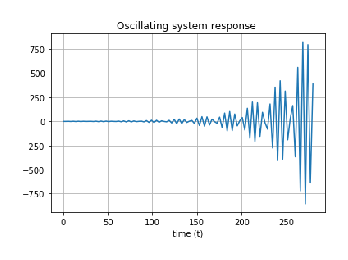
\includegraphics[width=\columnwidth]{./figs/es17btech11009/es17btech11009_1_1.eps}
\caption{}
\label{fig:es17btech11009_1_1}
\end{figure}
\begin{figure}[!ht]
\centering
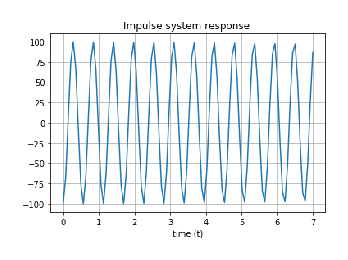
\includegraphics[width=\columnwidth]{./figs/es17btech11009/es17btech11009_imp.eps}
\caption{}
\label{fig:es17btech11009_imp}
\end{figure}
\renewcommand{\thefigure}{\theenumi}
\begin{table}[!ht]
\centering
%%%%%%%%%%%%%%%%%%%%%%%%%%%%%%%%%%%%%%%%%%%%%%%%%%%%%%%%%%%%%%%%%%%%%%
%%                                                                  %%
%%  This is the header of a LaTeX2e file exported from Gnumeric.    %%
%%                                                                  %%
%%  This file can be compiled as it stands or included in another   %%
%%  LaTeX document. The table is based on the longtable package so  %%
%%  the longtable options (headers, footers...) can be set in the   %%
%%  preamble section below (see PRAMBLE).                           %%
%%                                                                  %%
%%  To include the file in another, the following two lines must be %%
%%  in the including file:                                          %%
%%        \def\inputGnumericTable{}                                 %%
%%  at the beginning of the file and:                               %%
%%        \input{name-of-this-file.tex}                             %%
%%  where the table is to be placed. Note also that the including   %%
%%  file must use the following packages for the table to be        %%
%%  rendered correctly:                                             %%
%%    \usepackage[latin1]{inputenc}                                 %%
%%    \usepackage{color}                                            %%
%%    \usepackage{array}                                            %%
%%    \usepackage{longtable}                                        %%
%%    \usepackage{calc}                                             %%
%%    \usepackage{multirow}                                         %%
%%    \usepackage{hhline}                                           %%
%%    \usepackage{ifthen}                                           %%
%%  optionally (for landscape tables embedded in another document): %%
%%    \usepackage{lscape}                                           %%
%%                                                                  %%
%%%%%%%%%%%%%%%%%%%%%%%%%%%%%%%%%%%%%%%%%%%%%%%%%%%%%%%%%%%%%%%%%%%%%%



%%  This section checks if we are begin input into another file or  %%
%%  the file will be compiled alone. First use a macro taken from   %%
%%  the TeXbook ex 7.7 (suggestion of Han-Wen Nienhuys).            %%
\def\ifundefined#1{\expandafter\ifx\csname#1\endcsname\relax}


%%  Check for the \def token for inputed files. If it is not        %%
%%  defined, the file will be processed as a standalone and the     %%
%%  preamble will be used.                                          %%
\ifundefined{inputGnumericTable}

%%  We must be able to close or not the document at the end.        %%
	\def\gnumericTableEnd{\end{document}}


%%%%%%%%%%%%%%%%%%%%%%%%%%%%%%%%%%%%%%%%%%%%%%%%%%%%%%%%%%%%%%%%%%%%%%
%%                                                                  %%
%%  This is the PREAMBLE. Change these values to get the right      %%
%%  paper size and other niceties.                                  %%
%%                                                                  %%
%%%%%%%%%%%%%%%%%%%%%%%%%%%%%%%%%%%%%%%%%%%%%%%%%%%%%%%%%%%%%%%%%%%%%%

	\documentclass[12pt%
			  %,landscape%
                    ]{report}
       \usepackage[latin1]{inputenc}
       \usepackage{fullpage}
       \usepackage{color}
       \usepackage{array}
       \usepackage{longtable}
       \usepackage{calc}
       \usepackage{multirow}
       \usepackage{hhline}
       \usepackage{ifthen}

	\begin{document}


%%  End of the preamble for the standalone. The next section is for %%
%%  documents which are included into other LaTeX2e files.          %%
\else

%%  We are not a stand alone document. For a regular table, we will %%
%%  have no preamble and only define the closing to mean nothing.   %%
    \def\gnumericTableEnd{}

%%  If we want landscape mode in an embedded document, comment out  %%
%%  the line above and uncomment the two below. The table will      %%
%%  begin on a new page and run in landscape mode.                  %%
%       \def\gnumericTableEnd{\end{landscape}}
%       \begin{landscape}


%%  End of the else clause for this file being \input.              %%
\fi

%%%%%%%%%%%%%%%%%%%%%%%%%%%%%%%%%%%%%%%%%%%%%%%%%%%%%%%%%%%%%%%%%%%%%%
%%                                                                  %%
%%  The rest is the gnumeric table, except for the closing          %%
%%  statement. Changes below will alter the table's appearance.     %%
%%                                                                  %%
%%%%%%%%%%%%%%%%%%%%%%%%%%%%%%%%%%%%%%%%%%%%%%%%%%%%%%%%%%%%%%%%%%%%%%

\providecommand{\gnumericmathit}[1]{#1} 
%%  Uncomment the next line if you would like your numbers to be in %%
%%  italics if they are italizised in the gnumeric table.           %%
%\renewcommand{\gnumericmathit}[1]{\mathit{#1}}
\providecommand{\gnumericPB}[1]%
{\let\gnumericTemp=\\#1\let\\=\gnumericTemp\hspace{0pt}}
 \ifundefined{gnumericTableWidthDefined}
        \newlength{\gnumericTableWidth}
        \newlength{\gnumericTableWidthComplete}
        \newlength{\gnumericMultiRowLength}
        \global\def\gnumericTableWidthDefined{}
 \fi
%% The following setting protects this code from babel shorthands.  %%
 \ifthenelse{\isundefined{\languageshorthands}}{}{\languageshorthands{english}}
%%  The default table format retains the relative column widths of  %%
%%  gnumeric. They can easily be changed to c, r or l. In that case %%
%%  you may want to comment out the next line and uncomment the one %%
%%  thereafter                                                      %%
\providecommand\gnumbox{\makebox[0pt]}
%%\providecommand\gnumbox[1][]{\makebox}

%% to adjust positions in multirow situations                       %%
\setlength{\bigstrutjot}{\jot}
\setlength{\extrarowheight}{\doublerulesep}

%%  The \setlongtables command keeps column widths the same across  %%
%%  pages. Simply comment out next line for varying column widths.  %%
\setlongtables

\setlength\gnumericTableWidth{%
	48pt+%
	29pt+%
	85pt+%
0pt}
\def\gumericNumCols{3}
\setlength\gnumericTableWidthComplete{\gnumericTableWidth+%
         \tabcolsep*\gumericNumCols*2+\arrayrulewidth*\gumericNumCols}
\ifthenelse{\lengthtest{\gnumericTableWidthComplete > \linewidth}}%
         {\def\gnumericScale{\ratio{\linewidth-%
                        \tabcolsep*\gumericNumCols*2-%
                        \arrayrulewidth*\gumericNumCols}%
{\gnumericTableWidth}}}%
{\def\gnumericScale{1}}

%%%%%%%%%%%%%%%%%%%%%%%%%%%%%%%%%%%%%%%%%%%%%%%%%%%%%%%%%%%%%%%%%%%%%%
%%                                                                  %%
%% The following are the widths of the various columns. We are      %%
%% defining them here because then they are easier to change.       %%
%% Depending on the cell formats we may use them more than once.    %%
%%                                                                  %%
%%%%%%%%%%%%%%%%%%%%%%%%%%%%%%%%%%%%%%%%%%%%%%%%%%%%%%%%%%%%%%%%%%%%%%

\ifthenelse{\isundefined{\gnumericColA}}{\newlength{\gnumericColA}}{}\settowidth{\gnumericColA}{\begin{tabular}{@{}p{48pt*\gnumericScale}@{}}x\end{tabular}}
\ifthenelse{\isundefined{\gnumericColB}}{\newlength{\gnumericColB}}{}\settowidth{\gnumericColB}{\begin{tabular}{@{}p{48pt*\gnumericScale}@{}}x\end{tabular}}
\ifthenelse{\isundefined{\gnumericColC}}{\newlength{\gnumericColC}}{}\settowidth{\gnumericColC}{\begin{tabular}{@{}p{48pt*\gnumericScale}@{}}x\end{tabular}}

\begin{tabular}[c]{%
	b{\gnumericColA}%
	b{\gnumericColB}%
	b{\gnumericColC}%
	}

%%%%%%%%%%%%%%%%%%%%%%%%%%%%%%%%%%%%%%%%%%%%%%%%%%%%%%%%%%%%%%%%%%%%%%
%%  The longtable options. (Caption, headers... see Goosens, p.124) %%
%	\caption{The Table Caption.}             \\	%
% \hline	% Across the top of the table.
%%  The rest of these options are table rows which are placed on    %%
%%  the first, last or every page. Use \multicolumn if you want.    %%

%%  Header for the first page.                                      %%
%	\multicolumn{3}{c}{The First Header} \\ \hline 
%	\multicolumn{1}{c}{colTag}	%Column 1
%	&\multicolumn{1}{c}{colTag}	%Column 2
%	&\multicolumn{1}{c}{colTag}	\\ \hline %Last column
%	\endfirsthead

%%  The running header definition.                                  %%
%	\hline
%	\multicolumn{3}{l}{\ldots\small\slshape continued} \\ \hline
%	\multicolumn{1}{c}{colTag}	%Column 1
%	&\multicolumn{1}{c}{colTag}	%Column 2
%	&\multicolumn{1}{c}{colTag}	\\ \hline %Last column
%	\endhead

%%  The running footer definition.                                  %%
%	\hline
%	\multicolumn{3}{r}{\small\slshape continued\ldots} \\
%	\endfoot

%%  The ending footer definition.                                   %%
%	\multicolumn{3}{c}{That's all folks} \\ \hline 
%	\endlastfoot
%%%%%%%%%%%%%%%%%%%%%%%%%%%%%%%%%%%%%%%%%%%%%%%%%%%%%%%%%%%%%%%%%%%%%%

\hhline{|-|-|-}
	 \multicolumn{1}{|p{\gnumericColA}|}%
	{\gnumericPB{\centering}\gnumbox{\textbf{M in dB}}}
	&\multicolumn{1}{p{\gnumericColB}|}%
	{\gnumericPB{\centering}\gnumbox{\textbf{M}}}
	&\multicolumn{1}{p{\gnumericColC}|}%
	{\gnumericPB{\centering}\gnumbox{\textbf{$\omega$}}}
\\
\hhline{|---|}
	 \multicolumn{1}{|p{\gnumericColA}|}%
	{\gnumericPB{\centering}\gnumbox{13.64}}
	&\multicolumn{1}{p{\gnumericColB}|}%
	{\gnumericPB{\centering}\gnumbox{4.81}}
	&\multicolumn{1}{p{\gnumericColC}|}%
	{\gnumericPB{\centering}\gnumbox{1.68}}
\\
\hhline{|---|}
	 \multicolumn{1}{|p{\gnumericColA}|}%
	{\gnumericPB{\centering}\gnumbox{11.84}}
	&\multicolumn{1}{p{\gnumericColB}|}%
	{\gnumericPB{\centering}\gnumbox{3.91}}
	&\multicolumn{1}{p{\gnumericColC}|}%
	{\gnumericPB{\centering}\gnumbox{1.85}}
\\
\hhline{|---|}
	 \multicolumn{1}{|p{\gnumericColA}|}%
	{\gnumericPB{\centering}\gnumbox{7.64}}
	&\multicolumn{1}{p{\gnumericColB}|}%
	{\gnumericPB{\centering}\gnumbox{2.41}}
	&\multicolumn{1}{p{\gnumericColC}|}%
	{\gnumericPB{\centering}\gnumbox{1.98}}
\\
\hhline{|---|}
	 \multicolumn{1}{|p{\gnumericColA}|}%
	{\gnumericPB{\centering}\gnumbox{5.15}}
	&\multicolumn{1}{p{\gnumericColB}|}%
	{\gnumericPB{\centering}\gnumbox{1.81}}
	&\multicolumn{1}{p{\gnumericColC}|}%
	{\gnumericPB{\centering}\gnumbox{2.07}}
\\
\hhline{|---|}
	 \multicolumn{1}{|p{\gnumericColA}|}%
	{\gnumericPB{\centering}\gnumbox{-4.29}}
	&\multicolumn{1}{p{\gnumericColB}|}%
	{\gnumericPB{\centering}\gnumbox{0.61}}
	&\multicolumn{1}{p{\gnumericColC}|}%
	{\gnumericPB{\centering}\gnumbox{2.61}}
\\
\hhline{|---|}
	 \multicolumn{1}{|p{\gnumericColA}|}%
	{\gnumericPB{\centering}\gnumbox{-40}}
	&\multicolumn{1}{p{\gnumericColB}|}%
	{\gnumericPB{\centering}\gnumbox{0.01}}
	&\multicolumn{1}{p{\gnumericColC}|}%
	{\gnumericPB{\centering}\gnumbox{8.71}}

\\
\hhline{|-|-|-|}
\end{tabular}

\ifthenelse{\isundefined{\languageshorthands}}{}{\languageshorthands{\languagename}}
\gnumericTableEnd
\caption{}
\label{table:es17btech11009_Table1}
\end{table}
\item Verify your results using spice for the parameters given in Table \ref{table:es17btech11009_Table1}.
%Find the frequency for arbitrary R,C values as given in 
\solution 
The loop will oscillate at frequency $\omega_{o}$, given by
\begin{align}
    \omega_{o} = \frac{1}{RC}
%\end{align}
%From Table \ref{table:es17btech11009_Table1},
%\begin{align}
\\
 &= 20 rad/s
\\
\text{or, }
%\end{align}
%\begin{align}
    f &=  3.184 Hz
\label{eq:es17btech11009_f}
\end{align}
%
%
%\item
%Simulate the circuit Fig \ref{fig:es17btech11009_fig3} using spice simulators and plot the generated output using python script.

The following spice netlist generates the output
\begin{lstlisting}
spice/es17btech11009.net
\end{lstlisting}
which is plotted by the following python code  in Fig. \ref{fig:es17btech11009_spice}
%
\begin{lstlisting}
codes/es17btech11009/es17btech11009_spice.py
\end{lstlisting}
\begin{figure}[!ht]
\centering
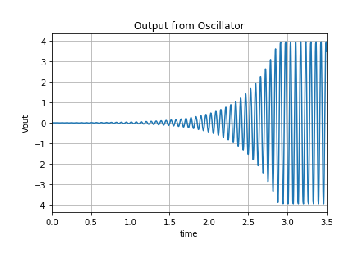
\includegraphics[width=\columnwidth]{./figs/es17btech11009/es17btech11009_spice.eps}
\caption{}
\label{fig:es17btech11009_spice}
\end{figure}
A zoomed version is plotted in Fig. \ref{fig:es17btech11009_spice1} by the following code.
%
%\item
%Consider part of the spice simulation and the following code plots the part of the output as shown in Fig \ref{fig:es17btech11009_spice1}
\begin{lstlisting}
codes/es17btech11009/es17btech11009_spice1.py
\end{lstlisting}
\begin{figure}[!ht]
\centering
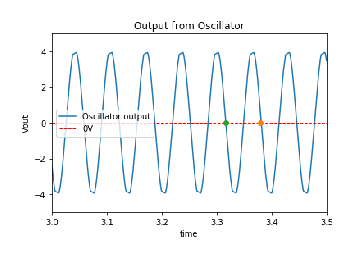
\includegraphics[width=\columnwidth]{./figs/es17btech11009/es17btech11009_spice1.eps}
\caption{}
\label{fig:es17btech11009_spice1}
\end{figure}
From Fig \ref{fig:es17btech11009_spice1},
Time period of oscillation 
\begin{align}
    T = 3.3801 - 3.317
\end{align}
\begin{align}
    f = \frac{1}{T} = 15.847 Hz
\end{align}
%\begin{align}
%    \omega_{o} = 2\pi f = 99.5 rad/s
%\end{align}
%
which is close to the theoretical value in \eqref{eq:es17btech11009_f}
%
%\begin{align}
%    \omega_{o} = 2\pi f = 19.8 rad/s
%\end{align}
%Hence the frequency calculated from the formulae and the plot are approximately same.
\end{enumerate}
